\section{The Intel 486}

\begin{wrapfigure}[5]{r}{0.25\textwidth}
\centering

\includegraphics[width=.25\textwidth]{drawings/intel_logo.pdf}
\end{wrapfigure}

Announced in 1989, the Intel 80486 was a performance evolution which addressed all bottlenecks of the 386. However it's pricetag of \$950 (\$1,920 in 2018) kept it away from most consumers. By 1993, the chip price had lowered to the point it was finally becoming affordable. It would become \doom recommended CPU.\\
\par
The design has changed significantly compared to its predecessor, the 486. The pipeline was gifted with two extra stages, extending its depth to five. The floating point unit which used to be optionnal and somewhere on the motherboard became mandatory and built-in. Most importantly manufacturing improvements allowed the 486 to have a decent size L1 cache.\\
\par
\fq{The 386 actually had small cache that eventually got exited because it didn't have enough performance for the size of the cache that we could put on board the chip, and the problem was if you made the chip bigger, it literally wouldn't fit inside the lithography machine's field of view, to flash on the chip}{Gene Hill - Intel 386 Microprocessor Design and Development}\\
\par

\drawing{486_arch}{Intel 486 architecture}
\par
Like for the 386, Intel marketed its new CPU in two flavors. A DX version which was the pure technology and a SX version which was "slower". But while it was a deliberate design choice to offer a 386 which was slower but more affordable, the 486 SX was in fact a trick. Due to manufacturing problems, the first 486 CPU came out of the factories working normally but with faulty FPUs units. Instead of throwing the faulty CPUs away, Intel sold them at a discounted (50\%) price and labeled them "SX"\footnote{Later on Intel fixed there production process but they kept offering the SX since most customers prefered getting a discount instead of a FPU they had little to no usage of}.\\
\par
If in retrospect the 486 was Intel's 1994 champion and an unquestionable powerhouse (both in terms of performances and sales\footnote{It was still manufactured as late as 2015 for routers}), it had to sustain a period of uncertaincy. Like the 386 had to face its brother (the XXX), the i486 also had to a competitor from the same company. Its archemesis name was Intel 860.\\
\par
\fq{

\begin{wrapfigure}[11]{r}{0.55\textwidth}
\centering
\scaledimage{0.55}{i860.png}
\end{wrapfigure}

...We now had two very powerful chips that we were introducing at just about the same time: the 486, largely based on CISC technology and compatible with all the pc software, and the i860, based on RISC technology, which was very fast but compatible with nothing. we didn't know what to do. so we introduced both, figuring we'd let the marketplace decide. however, things were not that simple. supporting a microprocessor architecture with all the necessary computer-related products --- software, sales, and technical support --- takes enormous resources. even a company like Intel had to strain to do an adequate job with just one architecture. and now we had two different and competing efforts, each demanding more and more internal resources. development projects have a tendency to want to grow like the proverbial mustard seed. the fight for resources and for marketing attention (for example, when meeting with the customer, which processor should we highlight) led to internal debates that were fierce enough to tear apart our microprocessor organization. meanwhile, our equivocation caused our customers to wonder what Intel really stood for, the 486 or i860?}{Andy Grove, "Only the paranoid survive".}
\bigskip
\par
In practice however the i860 never stood a chance. Relying on an heavily pipelined superscaler architecture crushing VLIWs\footnote{Very long instruction word.}. It three units, X, Y ,and Z allowed parallel processing which when efficently used allowed it to outperform the Intel 486.
But where later CPUs such as the Pentium chose to hide the chip complexity by automatically executing instruction in parralele when possible, the i860 architect allowed direct access to its parallel pipeline. The chip did nothing behind the scene and rely on compiler writers to sequence instructions appropriately.\\
\par
Unfortunately compiler technology was not there yet. Without Intel's full backing to generate the precious tool, none of the compilers available came even remotely close to generating instructions able to exploit its super scalar capability. the i860 was never able to reach its full potential. If only Intel had been willing to build the compilers it desperately needed the i860 history could have been different.\\
\par
\par
\trivia{Amusingly, the i860 would still play a part in Doom's development since it was used on NextDimension boards.}\\
\par
\cscaledimage{1}{i486DX.png}{The Intel 486 packing 1.2 millions transistors.}

\par
\subsection{Pipeline improvements}
Charting the 486 MIPs performances along with the previous generation make the performance boost appear vividly. If, thanks to manufacturing improvements, top of the line 486 were able to run at 50Mhz, the frequency increase was not the main factor of improvement.\\
\par
 Looking closely at the chart, one will notice that even at equal frequency, a 486 offered more than twice the processing power of a 386.\\

\par
\begin{figure}[H]
\centering
  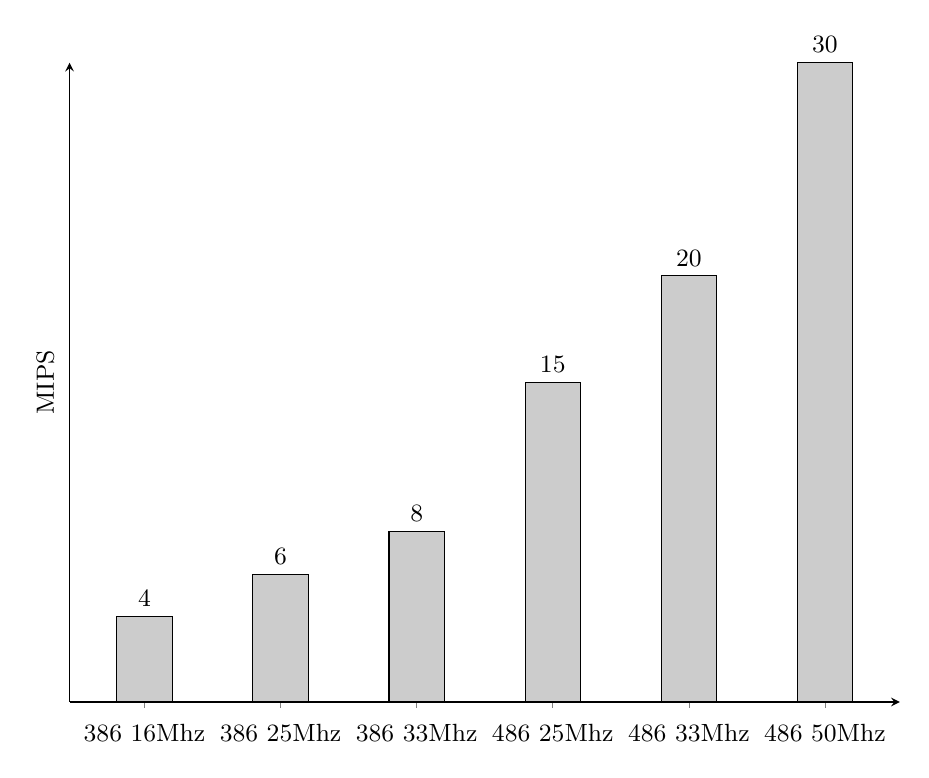
\begin{tikzpicture}[font=\small]
    \begin{axis}[
      width=1.0\textwidth,
      height=0.8\textwidth,
      ybar,
      bar width=20pt,
      ylabel={MIPS},
      ymin=0,
      ytick=\empty,
      xtick=data,
      axis x line=bottom,
      axis y line=left,
      enlarge x limits=0.11,
      symbolic x coords={386 16Mhz,386 25Mhz,386 33Mhz,486 25Mhz,486 33Mhz,486 50Mhz},
      xticklabel style={anchor=base,yshift=-\baselineskip},
      nodes near coords={\pgfmathprintnumber\pgfplotspointmeta}
    ]
      \addplot[fill=black!20,draw=black] coordinates {
        (386 16Mhz,4)
        (386 25Mhz,6)
        (386 33Mhz,8)
        (486 25Mhz,15)
        (486 33Mhz,20)
        (486 50Mhz,30)
      };
    \end{axis}
   
   \end{tikzpicture}
   \caption{Comparison\protect\footnotemark of Intel CPUs with MIPS \protect\footnotemark.}
 \end{figure}
\footnotetext{Source: "Roy Longbottom's PC Benchmark Collection: http://www.roylongbottom.org.uk/mips.htm".}

However since its frequency is the same as a 386, the 486 is unable to execute instructions faster. The way it achieves higher performances is through a higher average thoughput. According to its documentation the 386 was a smoothly three stage pipelined processor. Under ideal condition, figure \ref{386_doc_pipeline} shows how it should have in theory been able to execute one instruction per cycle. But under this neat diagram lied a serious bottleneck.\\
\par
\begin{figure}[H]
\centering
\includegraphics[width=\textwidth]{drawings/386_instruction_pipeline.pdf}
\caption{386 pipeline in Intel documentation.}
\label{386_doc_pipeline}
\end{figure}



\par
Even if the Prefetch Unit and the Execution Unit were properly fed, the Decode unit always took a minimum of two cycles to decode an instruction\footnote{The author speculates this high decode cost was the result of Intel's choice to use CISC instead of RISC.}. Since the maximum throughput of a pipeline cannot exceed the speed of its slowest stage, the Intel 386 could process at its most one instructions every two cycles.\\
\par

\begin{figure}[H]
\centering
\includegraphics[width=\textwidth]{drawings/actual_386_instruction_pipeline.pdf}
\caption{386 pipeline: Two cycles per instruction.}

\end{figure}

\par
To solve this problem, Intel simply decided to break the three stage pipeline into four (plus an other stage explained later). With all stages performing at 1 CPI, the total throughput of the 486 was doubled, which doubled perfomances (as long as the pipeline never starved).\\
\begin{figure}[H]
\centering
\includegraphics[width=\textwidth]{drawings/actual_486_instruction_pipeline.pdf}
\caption{486 pipeline: One cycle per instruction.}
\end{figure}
\par





\subsection{Caching }
Modifying the pipeline and make each stage run as fast as each others was one step in the right direction. But making the pipeline deeper also made it more vulnerable to starvation. Starting from an empty pipeline, the 486 had a latency of 5 cycles compared to the 486 which had only three stages.\\
\par
 A frequently stalling 486 would have been slower than a 386. As it would turn out, avoid starvation was difficult. Starting in 1980, RAM speed had started to lag behind CPU speed. By 1989, RAM access tme was 10 times slower than CPU.\\
\par
\pngdrawing{ram_vs_cpu}{}
\par
Until the 486, a CPU requesting either instructions or datas from the RAM always had to go through its Bus unit and communicate with the Bus which would route request to the RAM. As optimized as the protocol was took at the very minimum two cycles. One cycle to init the bus request, place the address on the address line and set the control line (Read/Write). And at least one wait cycle (which Intel called Wait State since while waiting on the Bus, the CPU did absolutely nothing).\\
\par
\pngdrawing{cpu_chipset_bus}{}
\par
If a device was able to answer the bus request within the first wait state, the CPU was able to resume operations, having reached a Zero Wait state. Otherwise, Wait States were inserted in order to wait for the request to complete. From a performance perspective, these WAIT STATEs were a disaster.\\\\
\par
\pngdrawing{cpu_wait_states}{}
The idea behind the L1 cache is to exploit both locality and temporality of code. Temporality is mainly a factor of code structure being made of loops. If an instruction is used, it is likely to be in a loop and be used sooner than later. Locality is also  factor of code structuring meaning that if an area of the RAM is accessed, it is likely a nearby other RAM area will also be accessed soon.\\
\par
By leverating these two properties, a cache located between the CPU and the Bus unit will often already contains the data requested, making a bus request useless. As a result, Intel engineers added an internal cache system sitting between the pipeline and the Bus Unit.\\
\par
\pngdrawing{cpu_cache}{}




\subsection{L1 Cache}
As we are making our way deep into Intel's technology it is now abundantly clear the cache is the cornerstone of the entire CPU. Without it there is no gain. Designing the cache to yeild the highest hit rate possbile and make it as fast as possible were paramount. 

\subsubsection{DRAM vs SRAM}
The first thing the cache had going on for itself is the lower latency of its RAM. If the main RAM on the SIMM slots used DRAM (Dymanic RAM) the cache was made of a different type called SRAM, able to  much faster access time. DRAM of these days typically had an access time of 150ns while SRAM was capable of 10ns, 150\% faster.\\
\par
DRAM was "slow" grealy because it was unavailable some of the time. The design of each cells was simple, based on one transistor and one storage capacitor. Two elements allowed for tight packing and hight capacity. The problem was with the capacitor losing its charge over time. The only way to keep the RAM integrity was to periodically refresh it every 15$\mu s$, by sending current into the capacitor. While the refresh happened, the bit cell was unavailable.\\
\par
\spngdrawing{0.5}{DRAM}{Dynamic RAM}
The DRAM also had the disavantage to be far away. Located "somewhere" on the motherboard so to access it, the CPU had to request it to its Bus Unit. Not only that was far away (in terms of physical distance), the bus had to be shared with other I/O devices.\\
\par
A different type of ram would solve all these problem. It is called SRAM.\\
\par
\spngdrawing{0.5}{SRAM}{Static RAM}
\par
Located inside the chip, accessing it did not require an expensive bus request. Moreover it was designed differently with no less than six transistors which did not need periodic refresh.
\par










\subsubsection{Cachelines}
Not only the L1 cache was made of faster RAM, it was also cleverly design. Its small size (8 KiB) and heavy duty (unified cache for both code and data) placed a considerable stress on its design. Nonetheless it managed an impressive 92\% hit rate\footnote{Source: "The i486 CPU: Executing Instructions in One Clock Cycle".} under normal operation.\\
\par
To achieve this, Intel engineers used a four-way associative design where the $2^{32}$ address space is divided in 1,953,125 pages of 2 KiB. Within each page, 128 lines of 16 bytes (called cacheline).\\
\par
\drawing{cacheline}{The 16 bytes in a cacheline.}
\par
The cache system is made of one directory and four banks (also called ways). Each way can store 128 cacheline and therefore has a capacity of 2 KiB. These lines of 16 bytes are the elementary unit of the cache. It only deals with what it calls cachelines.\\
\drawing{mem_to_way}{How a memory address is interpreted by the cache controller}
\par
Upong receiving a 32-bit address access request, the cache controller splits it in three fields.
\begin{enumerate}
\item Use the LINE field [4-11] to look up one of the 128 dictionary entries.
\item Look at the four tags in the entry, if one matches the TAG [12-31] then it means the cacheline is present in one of the four ways.
\item Check the flag F in the directory to make sure the cacheline is valid.
\item With the way ID known, use the OFFSET [0-3] field to access the value in the cacheline.
\item Update the flag F in the directory entry to update the LRU value.
\end{enumerate}
\par
If a value was to be written an all cacheline in the four ways are valid, the cache controller uses a LRU\footnote{Least Recently Used} to evict a cacheline.\\
\par
\drawing{cacheways}{The cache controller and its four ways (banks).}
%This design allowed code and data to node evict each others in loop. The fact that four ways were rotated with LRU made this cache very efficient.\\
\par
\trivia{What about increasing the number of ways? What about the cache size? An8 KiB four ways grant the best trade-off\footnote{Computer Architecture: A Quantitative Approach}. A two ways cache yields a 14\% miss rate, a four-ways 10.5\% hit rate but going to eight only improves the percentage to 10\% and fully associative to 9\%. The decreasing return on investment appears vividly once one a graph.}\\
\par


  \begin{figure}[H]
    \centering
    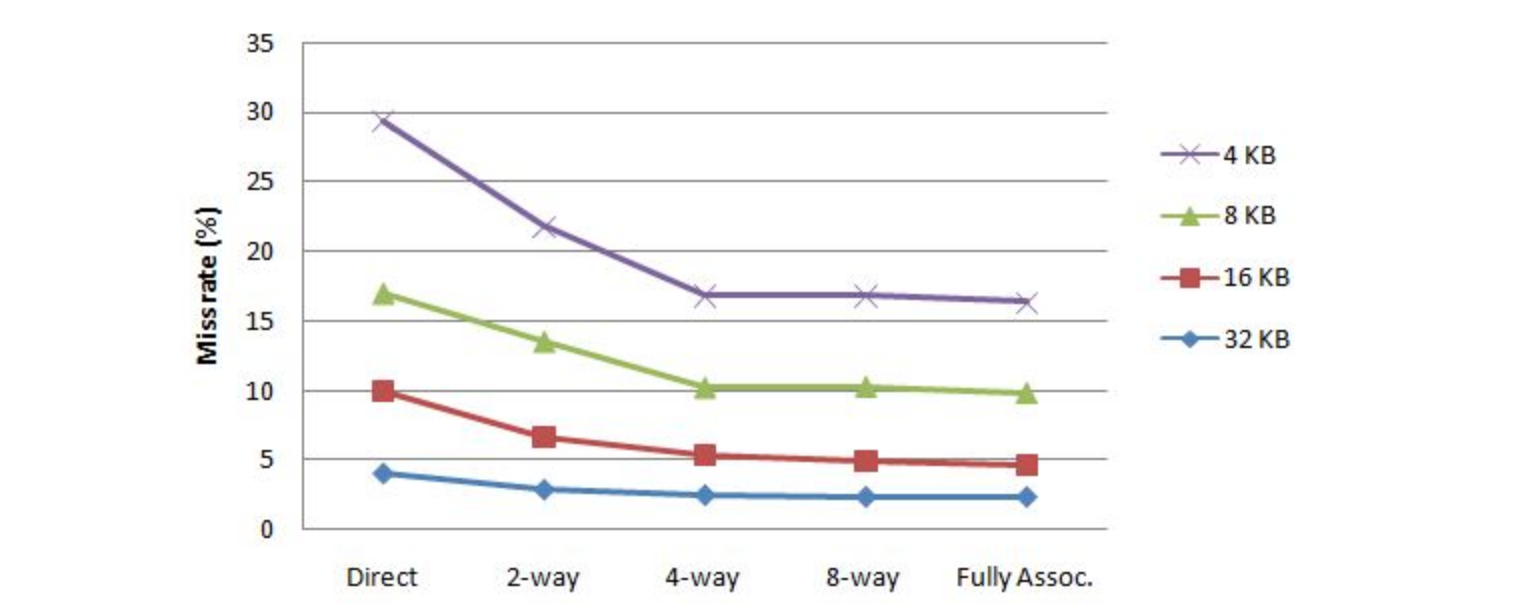
\includegraphics[width=0.9\textwidth]{drawings/set_cache_stats.png}
    \caption{}
  \end{figure}
  \par


\subsection{Netburst}
Any cache miss within the 486 pipeline triggered the eviction of a cacheline and a full 16 bytes had to be transfered from DRAM to SRAM\footnote{The prefetcher also worked with units of 16 bytes. It retrieved and stored cacheline into a prefetch queue of 32 bytes.}. Normally this would have been a very costy operation and a huge issue for the CPU. But Intel added something called NetBurst capacity to make it all work together.\\
\par
Hit rate, ZERO WAIT STATE\\
\par
\pngdrawing{netburst}{NetBurst allows for 65\% faster cacheline filling.}







\subsection{Overdrive and Writeback}
As if the huge performance improvement of the 486 were not enough, Intel managed to top it all with the its line of 80486 OverDrive. These CPU featured a frequency multiplied which made them run two times faster than the bus\footnote{To this day, designers still try to solve the problem of having a CPU so much faster than the bus.}. The 33Mhz model CPU ran at 66Mmhz and was the golden standard until 1995. It was commonly called DX2-66 and was the absolute best to run \doom.\\
\par 
\drawing{486dx2_notm}{The best CPU to run \doom at the time.}
\par
%\trivia{Want even more performance? Not only a DX2-66 ran faster, they also came with an enhanced writeback L1 cache\footnote{The standard 486 L1 cache was writethrough with post-writes.}}

\begin{figure}[H]
\centering
  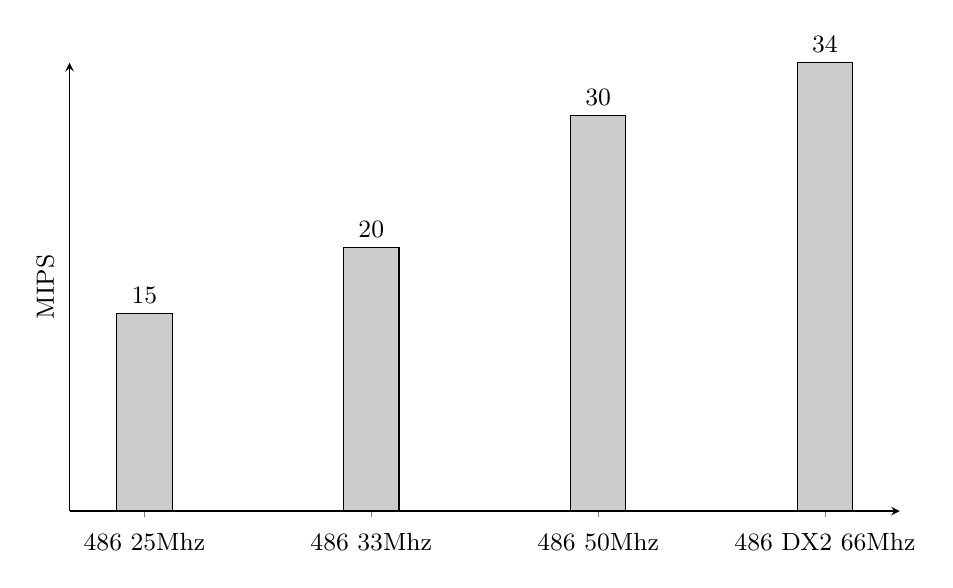
\begin{tikzpicture}[font=\small]
    \begin{axis}[
      width=1.0\textwidth,
      height=0.6\textwidth,
      ybar,
      bar width=20pt,
      ylabel={MIPS},
      ymin=0,
      ytick=\empty,
      xtick=data,
      axis x line=bottom,
      axis y line=left,
      enlarge x limits=0.11,
      symbolic x coords={486 25Mhz,486 33Mhz,486 50Mhz,486 DX2 66Mhz},
      xticklabel style={anchor=base,yshift=-\baselineskip},
      nodes near coords={\pgfmathprintnumber\pgfplotspointmeta}
    ]
      \addplot[fill=black!20,draw=black] coordinates {
        (486 25Mhz,15)
        (486 33Mhz,20)
        (486 50Mhz,30)
        (486 DX2 66Mhz,34)
      };
    \end{axis}
   
   \end{tikzpicture}
   \caption{Comparison\protect\footnotemark of CPUs with MIPS \protect\footnotemark.}
 \end{figure}
\footnotetext{Source: "Roy Longbottom's PC Benchmark Collection: http://www.roylongbottom.org.uk/mips.htm".}
\par
\trivia{Notice how a 486DX2-66Mhz is faster than a 485DX-50Mhz but not the full 20\% frequency could have made us expect. This is because the DX2 bus runs at 33Mhz while on the DX the CPU and the bus run at 50Mhz.}




\subsection{Die}
%To close this section on the 486, I cannot resist including a magnified photography of the die. 
If you are holding a physical 9.25''x7.5'' of this book, the CPU casing should be 30mm square and the die should be 15.5 x 9.9 mm at 1:1 scale.\\
\par
\bigskip

  \begin{figure}[!htb]

\begin{minipage}{0.48\textwidth}
\centering
\scaledrawimage{44.45mm}{486topdown.png}
%\caption{468 packaging.}
\end{minipage}
\hfill
\begin{minipage}{0.48\textwidth}
\centering
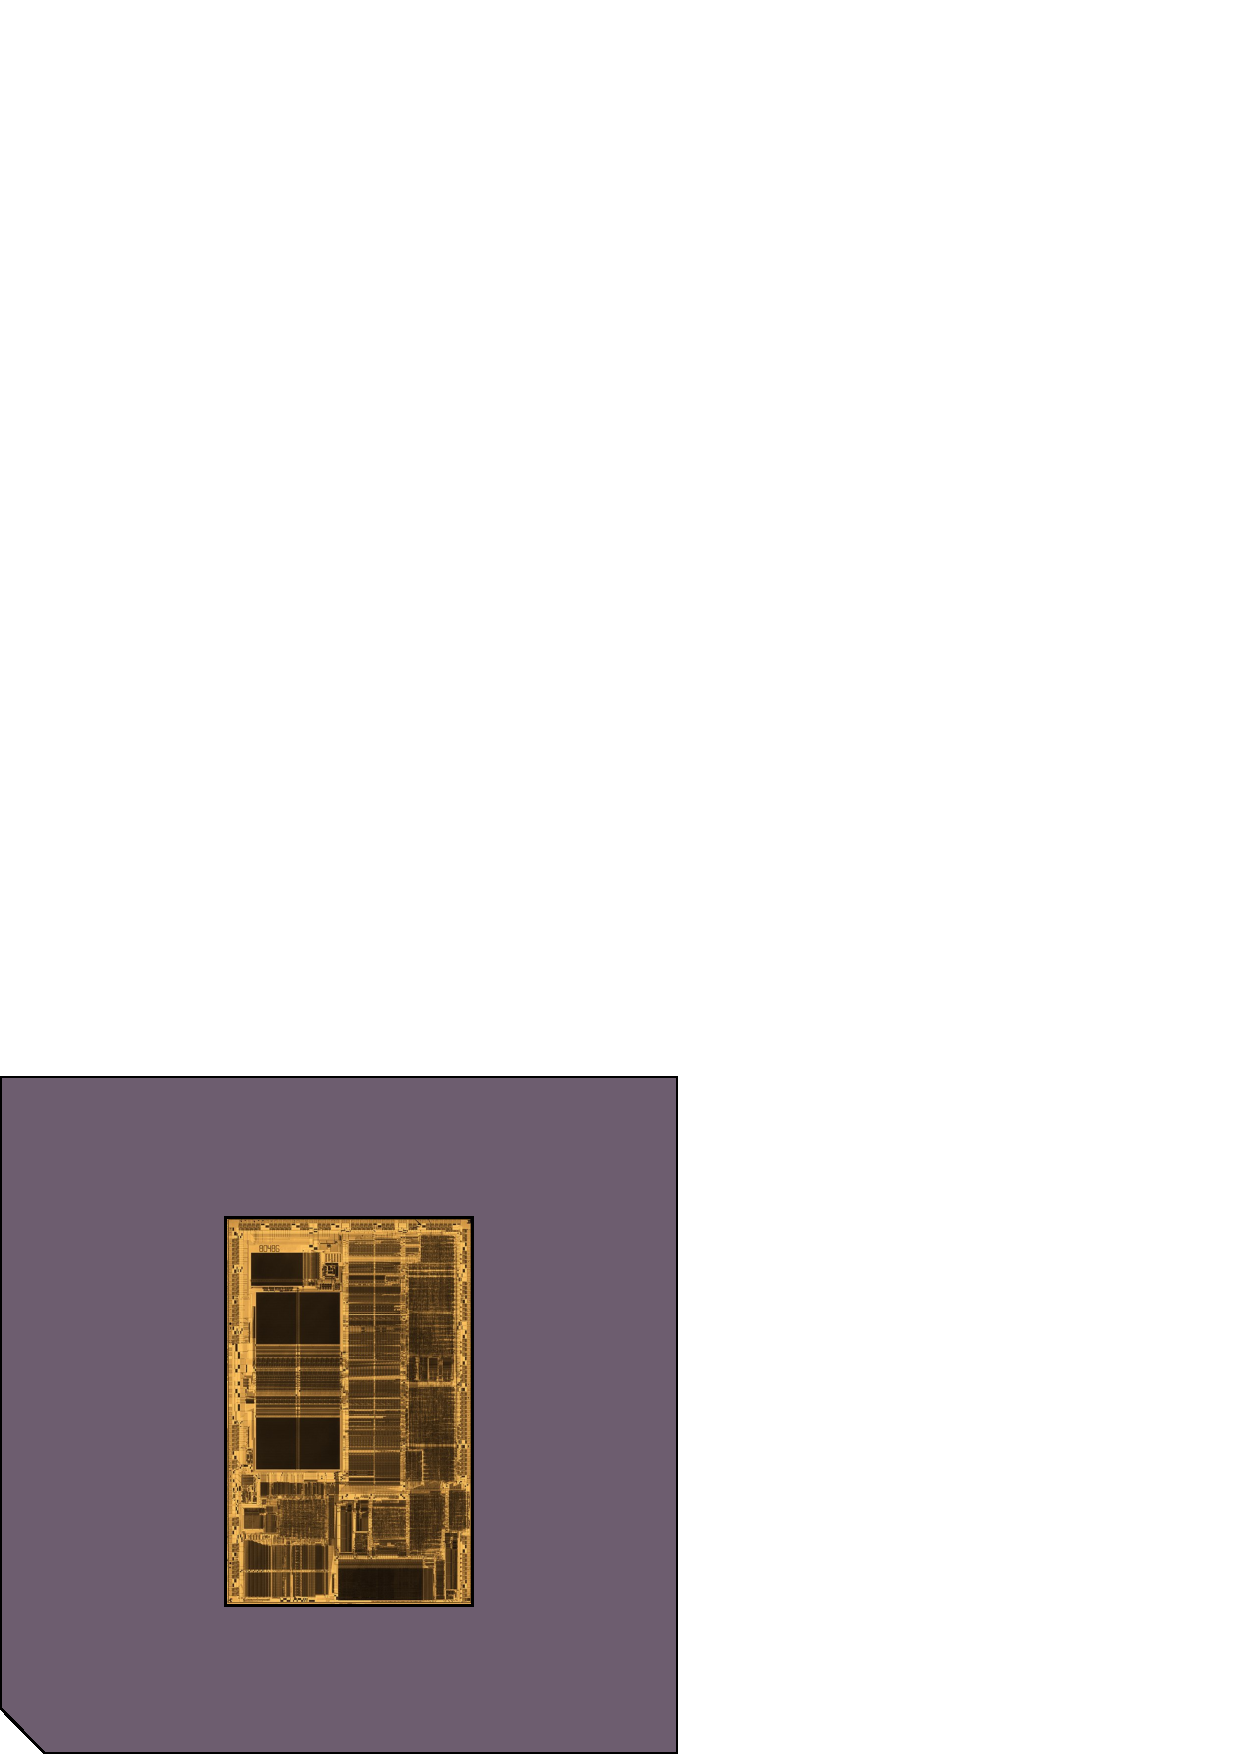
\includegraphics[width=44.45mm]{drawings/486toscale.pdf}
%\caption{The die inside the package.}
\end{minipage}
\end{figure}

\par



\begin{figure}[H]
\centering
\scaledimage{0.9}{486_blueprint.png}
\end{figure}
\par
\begin{figure}[H]
\centering
\scaledimage{0.9}{486_layout.png}
\end{figure}






\subsection{Programming the 486}
With the architecture in mind we can now understand how a programmer could take best advantage of the 486. The good news was most of the performance improvement was the characterized free-lunch of the 90s and 2000s. The exact same binary will run twice as fast on the new CPU.\\
\par
As long as the programer was mindful of the cacheline and maxmized time and space locality\footnote{And avoid branching, the 486 had no branch predictor. A \cw{jmp} instruction was a guaranteed pipeline flush}, the CPU would fly. That is for integers. Because as improved as the floating point unit was, it was still a far cry compared to the performance of the ALU and Barrel shifter.\\
\par
\begin{figure}[H]
\centering
\begin{tabularx}{\textwidth}{ X  X X  X  X}
  \toprule
  \textbf{CPU} & \textbf{FADD} & \textbf{FMUL} & \textbf{FDIV} &\textbf{FXCH} \\ \bottomrule
Intel 387 & 23-34 & 29-57   & 88-91 & 18 \\
Intel 487 & 8-20  & 16   & 73 & 4 \\ \bottomrule
\end{tabularx}
\caption{FPU performance: 387 vs 487.}

\end{figure}




\par
 \begin{figure}[H]
\centering  
\begin{tabularx}{\textwidth}{ L{0.3} L{0.3} L{0.4}}
  \toprule
  \textbf{Operation} &  \textbf{i486 (ALU)} & \textbf{i487 (FPU)} \\
  \toprule 
   
   \cw{ADD} & 1 & 8-20\\
   \cw{DIV} & 43 & 73\\
   \cw{MUL} & 12-42 & 29-52\\
   \toprule
\end{tabularx}
\caption{Comparaison ALU vs FPU operations.}
\end{figure}
\par
\trivia{There were many discussions on \cw{alt.games.doom} BBS\footnote. One endless thread in particular debated on what to get to play \doom. Should customer go for an SX, should they go for a DX which was supposed to be "faster"\footnote{\cw{alt.games.doom}: Does a 486DX run Doom faster than an SX?}. Comparing simple instruction speed for \cw{integer} and \cw{float} gives us the answer.}\\
 \par


The i386 was able to talk to an i387 located on the motherboard. Requests and responses had to transition on the bus and incurred four CPU cycles of overhead. For the i486, Intel decided to integrate the i487 FPU in the same die and improved performance by a factor 2.\\
\par
TODO: Drawing
\par

TODO: Verify with 387/487 description
TODO: How to program it? Use the cache luke and avoid branching. Re-read michael abrash guide on 486.
Full CPU Diagram.
Programming a 486\\
\par


alt.games.doom thread "Does a 486DX run Doom faster than an SX?" shows how hard it was to access information back then.\\

\fq{My friend is buying a computer and doesn't see much reason to buy
a DX.  Any opinions?  (or hard facts :) ?)}{Dave Gates}
\par
\fq{An SX is considerably slower than a DX for most processor-intensive
applications and games, including DOOM.}{Neal W.Miller}

\par
\fq{Thats wrong !
A 486 SX runs Doom with exactly the same speed like a 486 DX
(if you use the same VGA Card and Motherboard).}{Grassl Wolfgang}

\par
\fq{We have a 486SX/25 and a 486DX/50 and the DX 50 runs faster at full screen
high detail then the SX runs at postage stamp. It is so slow as to be
almost unplayable. }{BonesBro}
\par

\fq{DOOM runs *MUCH* faster on a 486DX/33 than on a 486SX/33.  Believe me,
I've seen it running on the 2 different machines in the same room.}{BillyBoB 4}
\par

\fq{They are *NOT* any different as far as CPU speed go.  Period.
The reason one (DX) is faster must have something to do with
probably the SX has an ISA video card, or no cache, or less
memory. Doom does NOT NOT NOT NOT use an FPU (math coprocessor) so there will be no slowdown for the SX.\\}{Chad Anson}





